\lecture{1}{07-07-2023}{1. The Geometry of Linear Equations}

\section{Initial Info}
These notes are for MIT 18.06 Linear Algebra, Spring 2005 tought by Gilbert Strang.

Linear algebra is about solving systems of linear equations.

\begin{align*}
    2x - y &= 0 \\
    -x +2y &= 3 
\end{align*}
These equations written in a matrix form:

\[
\left[ 
\begin{array}{cc}
    2 & -1 \\
    -1 & 2 
\end{array}
\right] 
\left[ 
\begin{array}{c}
    x \\
    y 
\end{array}
\right] = \left[ 
\begin{array}{c}
    0 \\
    3 
\end{array}
\right] 
\] 

\[ A  X = b .\] 

\begin{center}
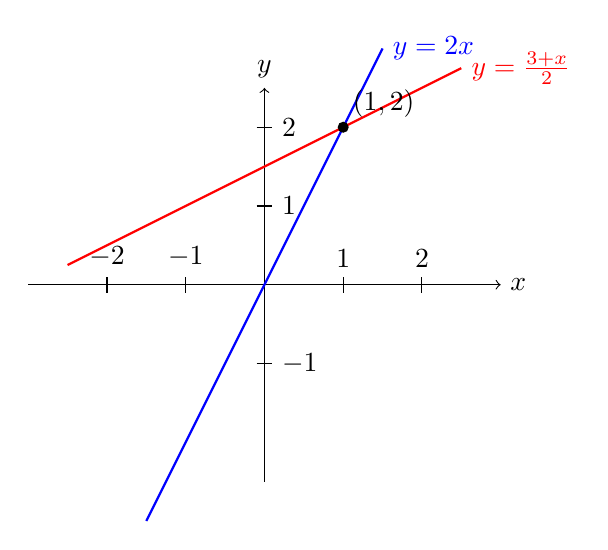
\begin{tikzpicture}[scale=1]
    % Axes
    \draw[->] (-3, 0) -- (3, 0) node[right] {$x$};
    \draw[->] (0, -2.5) -- (0, 2.5) node[above] {$y$};

    % Line 1: 2x - y = 0 (or y = 2x)
    \draw[blue, thick, domain=-1.5:1.5, samples=10] plot (\x, {2*\x}) node[right] {$y = 2x$};

    % Line 2: -x + 2y = 3 (or y = (3+x)/2)
    \draw[red, thick, domain=-2.5:2.5, samples=10] plot (\x, {(3+\x)/2}) node[right] {$y = \frac{3+x}{2}$};


    % Intersections
    \coordinate (intersection) at (1, 2);
    \fill[black] (intersection) circle (2pt) node[above right] {$(1, 2)$};

    % Grid
    %\draw[gray, dashed] (-2, -1.5) grid (2, 2);

    % Label for grid
    \foreach \x in {-2, -1, 1, 2}
    \draw (\x, -0.1) -- (\x, 0.1) node[above] {$\x$};
    \foreach \y in {-1, 1, 2}
    \draw (-0.1, \y) -- (0.1, \y) node[right] {$\y$};
\end{tikzpicture}
\end{center}



\nt{Giving up for now, this lin-alg tikz, matrix bs is not making sense in latex}

%\[ \atrix{cc|c}{
    %2 & -1 & 0 \\
    %%-1 & 2 & 3 
%} \]
